\documentclass{article}

\usepackage{graphicx}
\usepackage{tikz}
\usepackage{tikzsymbols}
\usetikzlibrary{calc,patterns,shapes.geometric}
\pagestyle{empty}
\usepackage[margin=0pt]{geometry}
\geometry{papersize={14in,12in}}

\def\centerarc[#1](#2)(#3:#4:#5){\draw[#1] ($(#2)+({#5*cos(#3)},{#5*sin(#3)})$) arc (#3:#4:#5);}

\begin{document}
	\begin{figure}
		\centering
		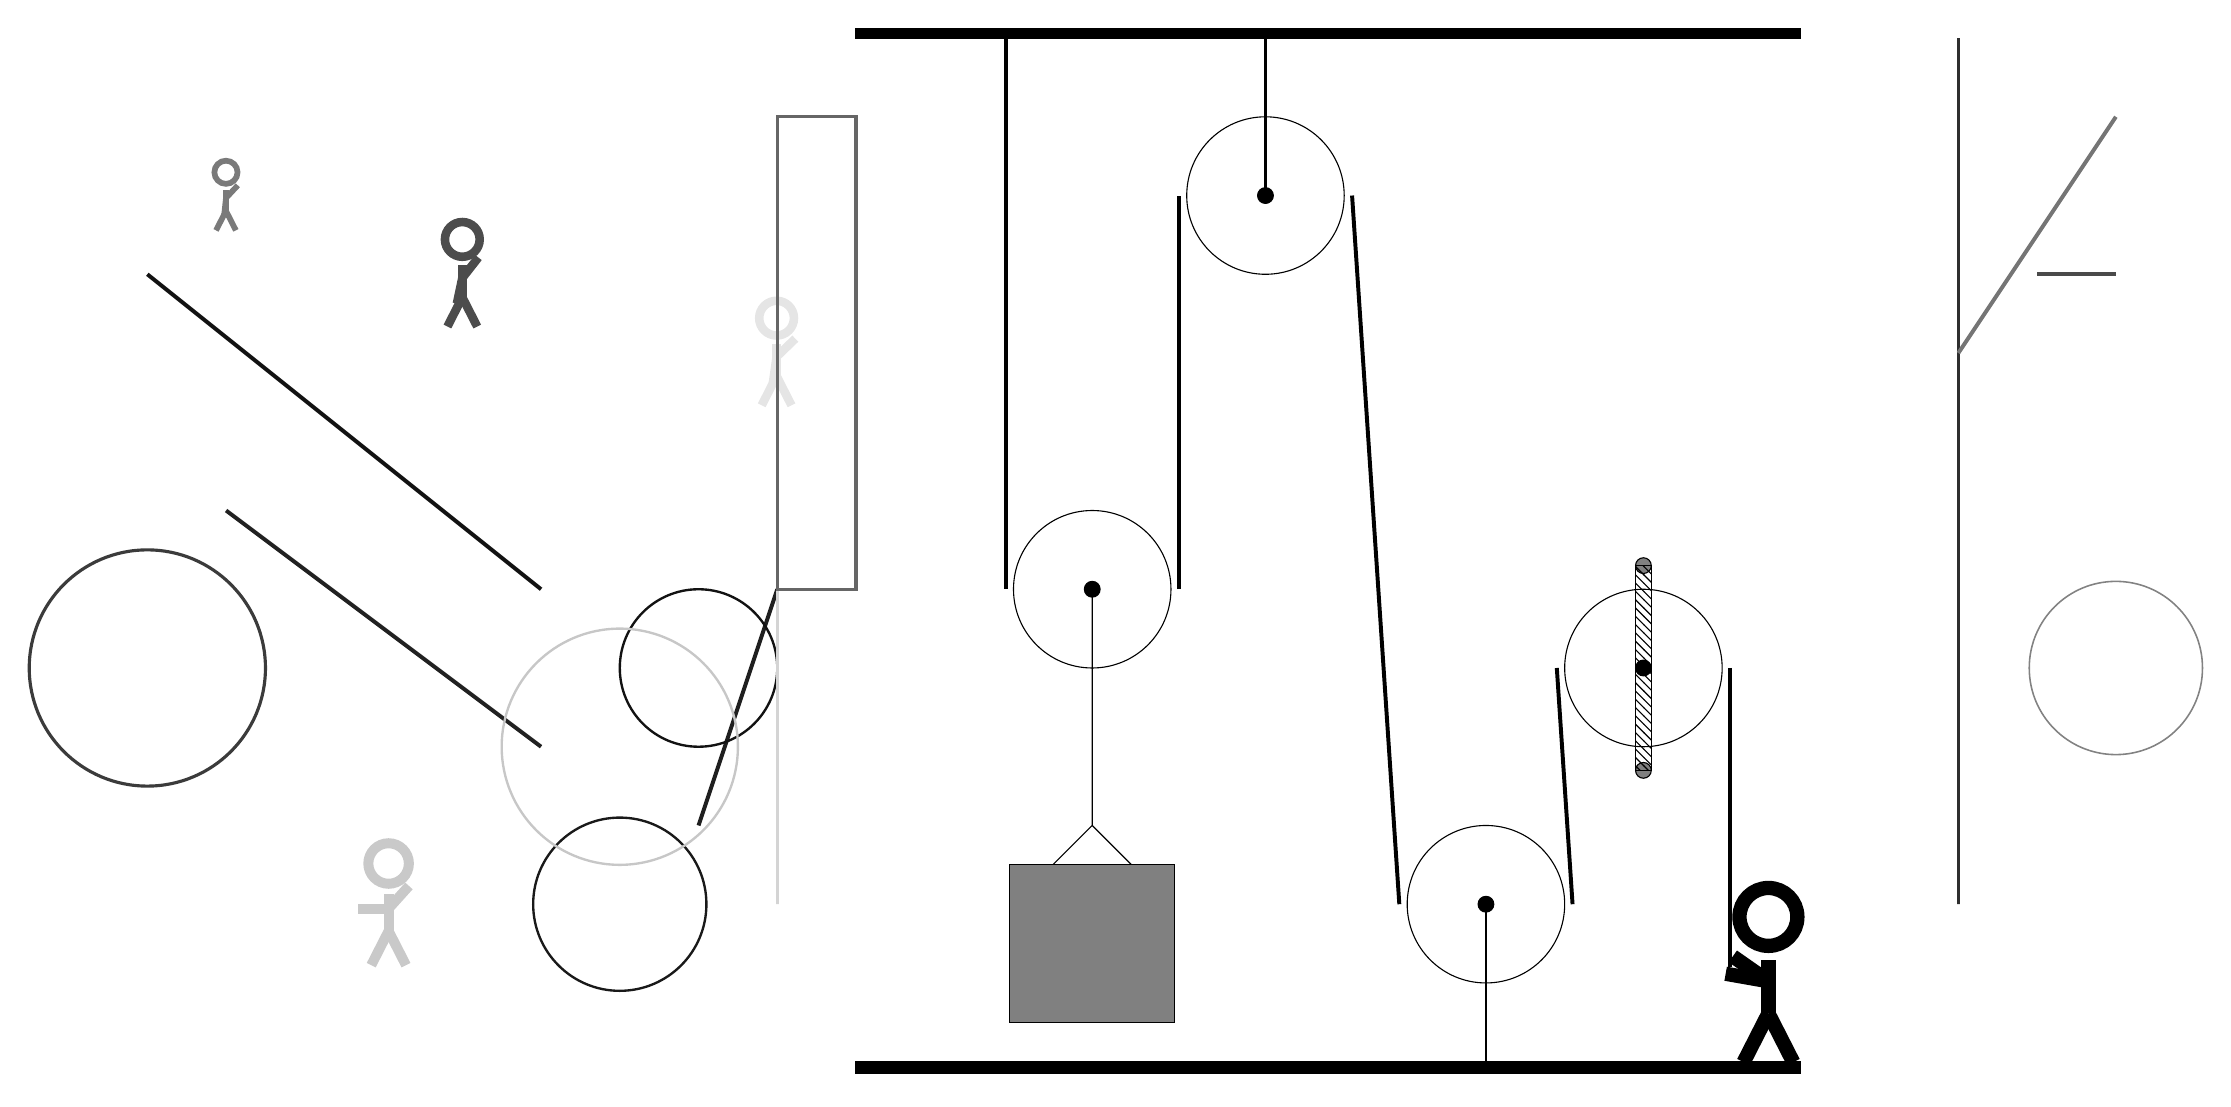
\begin{tikzpicture}
			%%%%% START %%%%%
			
			\draw[fill=black] (-2, 10) rectangle (10, 10.125);
			
			\draw (1, 3.0) circle (1);
			\draw[fill=black] (1, 3.0) circle (0.1);
			
			\draw (3.2, 8.0) circle (1);
			\draw[fill=black] (3.2, 8.0) circle (0.1);
			\draw[thick] (3.2, 8.0) -- (3.2, 10);
			
			\draw[line width=0.5mm, color=black!71](13, 7) -- (14, 7);
			
			\draw[line width=0.4mm, color=black!16] (12, 6) rectangle (12, 3);
			\draw [line width=0.2mm, color=black!49](14, 2) circle (1.1);
			\draw[line width=0.4mm, color=black!82] (12, -1) rectangle (12, 10);
			
			\node[line width=0.5mm, color=black!70] at (-7, 7) {\Strichmaxerl[6][78][52]};
			
			\draw [line width=0.4mm, color=black!77](-11, 2) circle (1.5);
			
			\draw[line width=0.5mm, color=black!54](14, 9) -- (12, 6);
			\draw[line width=0.5mm, color=black!88](-3, 3) -- (-4, 0);
			\draw[line width=0.5mm, color=black!87](-6, 1) -- (-10, 4);
			\draw[line width=0.5mm, color=black!93](-6, 3) -- (-11, 7);
			
			\draw [line width=0.3mm, color=black!93](-4, 2) circle (1.0);
			\draw[line width=0.4mm, color=black!17] (-3, -1) rectangle (-3, 3);
			\node[line width=0.2mm, color=black!21] at (-8, -1) {\Strichmaxerl[7][0][48]};
			
			\draw [line width=0.3mm, color=black!90](-5, -1) circle (1.1);
			\node[line width=0.7mm, color=black!10] at (-3, 6) {\Strichmaxerl[6][82][44]};
			\draw[line width=0.4mm, color=black!60] (-2, 9) rectangle (-3, 3);
			
			\node[line width=0.5mm, color=black!52] at (-10, 8) {\Strichmaxerl[4][84][47]};
			
			\draw [line width=0.3mm, color=black!22](-5, 1) circle (1.5);
			
			\draw (6, -1) circle (1);
			\draw[fill=black] (6, -1) circle (0.1);
			\draw[thick] (6, -1) -- (6, -3);
			
			\draw[fill=white](8, 2.0) circle (1);
			\draw[fill=black] (8, 2.0) circle (0.1);
			\draw[fill=black!50] (8, 3.3) circle (0.1);
			\draw[fill=black!50] (8, 0.7) circle (0.1);
			\draw[pattern=north west lines, pattern color=black] (7.9, 3.3) rectangle (8.1, 0.7);
			
			\draw (1, 3.0) -- (1, 0) -- (0.5, -0.5);
			\draw (1, 0) -- (1.5, -0.5);
			\draw[fill=black!50] (-0.05, -0.5) rectangle (2.05, -2.5);
			
			\draw[line width=0.5mm] (-0.1, 10) -- (-0.1, 3.0);
			\centerarc[line width=0.5mm](1, 3.0)(180:360:1.1);
			\draw[line width=0.5mm](2.1, 3.0) -- (2.1, 8.0);
			\centerarc[line width=0.5mm](3.2, 8.0)(0:180:1.1);
			\draw[line width=0.5mm](4.3, 8.0) -- (4.9, -1);
			\centerarc[line width=0.5mm](6, -1)(180:360:1.1);
			\draw[line width=0.5mm](7.1, -1) -- (6.9, 2.0);
			\centerarc[line width=0.5mm](8, 2.0)(0:180:1.1);
			\draw[line width=0.5mm](9.1, 2.0) -- (9.1, -1.8);
			
			\node at (9.5, -1.9) {\Strichmaxerl[10][-35][170]};
			
			\draw[fill=black] (-2, -3) rectangle (10, -3.15);
			
			%%%%% END %%%%%
		\end{tikzpicture}
	\end{figure}	
\end{document}